\documentclass[UTF8]{ctexart}

\usepackage{subfiles}  

%下面的语句, 引入你的头部设置文件
\usepackage{C:/phpStorm_proj/02_myself_ID_EGO/+100_latex_all_math_sel/myPreamble} 
%必须是绝对路径,才能让各个tex在单独编译时使用到

\title{文件名}


%---------------------------------


\begin{document}
	\tableofcontents % 生成目录
	\date{} % 若不写这句, 则默认也会渲染出日期, 所以我们要手动赋空值
	\maketitle  %这行代码, 让你前面的 title, author, date生效
	
	
	\part{t 检验}
	
	\section{中心极限定理 : 对一个总体, 进行大量重复的抽样. 将每次抽样的均值, 在横坐标轴上从小到大排开,并用柱状图表示``频次". 最终得到的柱状图的轮廓, 是一个``正态分布". 而且``对称轴"所标示的值,便是总体的``实际平均值$\mu$".}
	
	\begin{myEnvSample}
		一个学校有5000名学生, 某次学科考试, 假设我们无法获得到全部学生的成绩, 只能抽样获取部分人的成绩. 那我们能从部分人的成绩的平均值中, 来推测出全部5000人平均成绩吗? \\
				
		比如, 我们每次抽取20个学生的成绩, 算出20人成绩的平均数.\\		
		- 第一次抽20人, 假设算出该组(该样本)的平均成绩是 138分, 我们就在坐标轴的 x=138处, 放一个高度为1的矩形. 这里的高度1, 就代表"频数", 即目前, 138分, 出现1次. \\
		
		- 第二次抽20人,  假设算出该组的平均成绩依然是 138分, 现在, 138分就出现两次了, 这个值的频数就变成了2. \\
						
		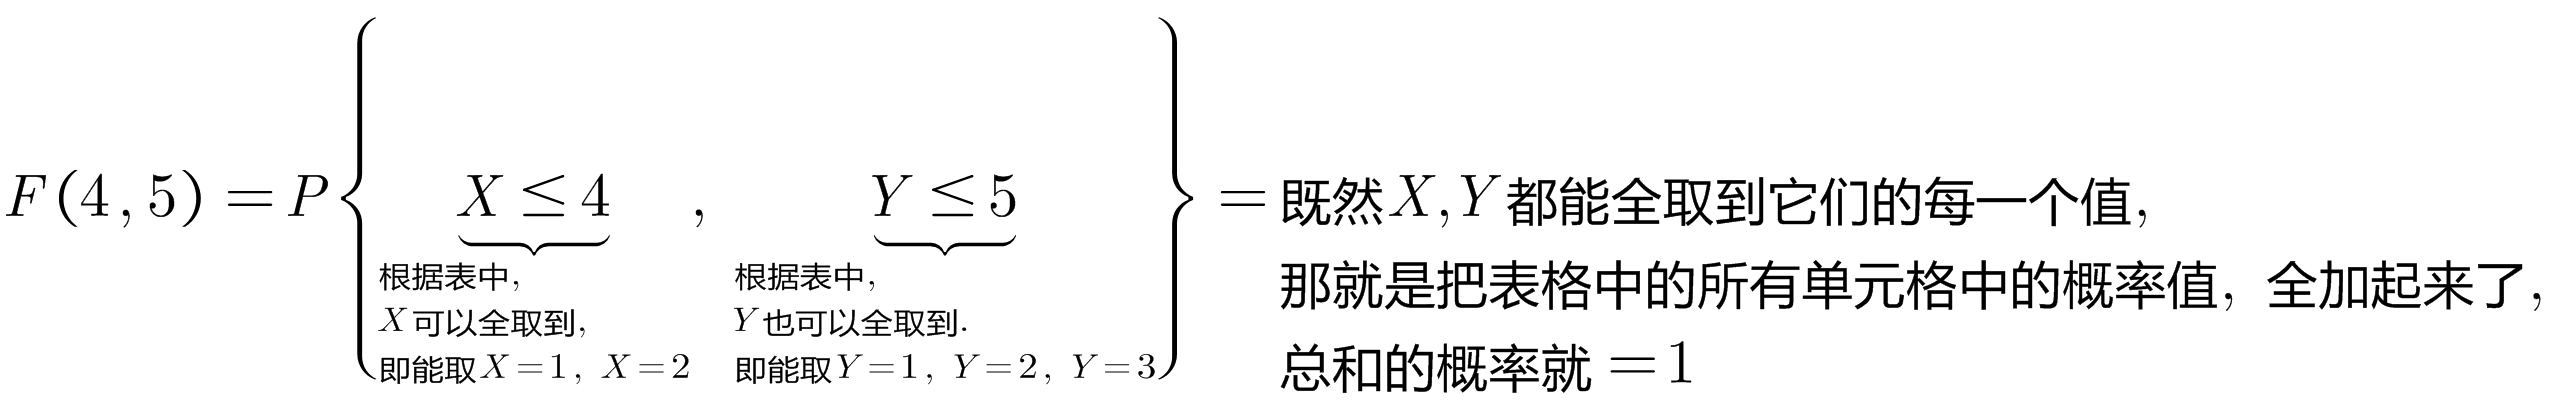
\includegraphics[width=0.55\textwidth]{/0222.png} \\
		
		我们抽样1000次(1000组), 每次20人, 并算出这20人的平均数, 放在坐标系上. 不同的平均分, 要统计相应的频数(该平均数出现的次数). \\
		1000次后, 我们就得到了一个呈现``正态分布"的结果. 我们把这条曲线的轮廓, 叫做``抽样分布". 这条曲线的对称轴, 在 137-138分之间. \\
				
		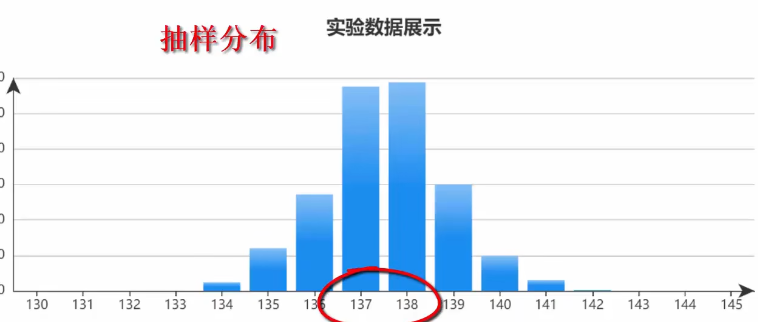
\includegraphics[width=0.7\textwidth]{/0223.png} \\		
		
		然后, 我们在excel表里面, 计算一下全校5000人的实际分数的平均值, 是 137.41分. 这表明, 我们从``抽样分布"中得到的对称轴处的数字, 非常精确于实际的平均值的数字.
		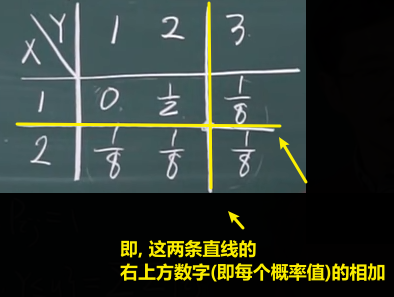
\includegraphics[width=0.25\textwidth]{/0224.png} \\			
		
		这个规律, 其实反映出的, 就是\textbf{``中心极限定理"}(其中的一个版本):  \\
		\textbf{对一个总体, 进行大量重复的抽样. 将每次抽样的均值, 在横坐标轴上从小到大排开,并用柱状图表示``频次". 最终得到的柱状图的轮廓, 是一个``正态分布". 而且``对称轴"所标示的值,便是总体的``实际平均值$\mu$".} \\
		
		如果把``抽样分布曲线"下的面积, 记作100\%. 则有: \\
		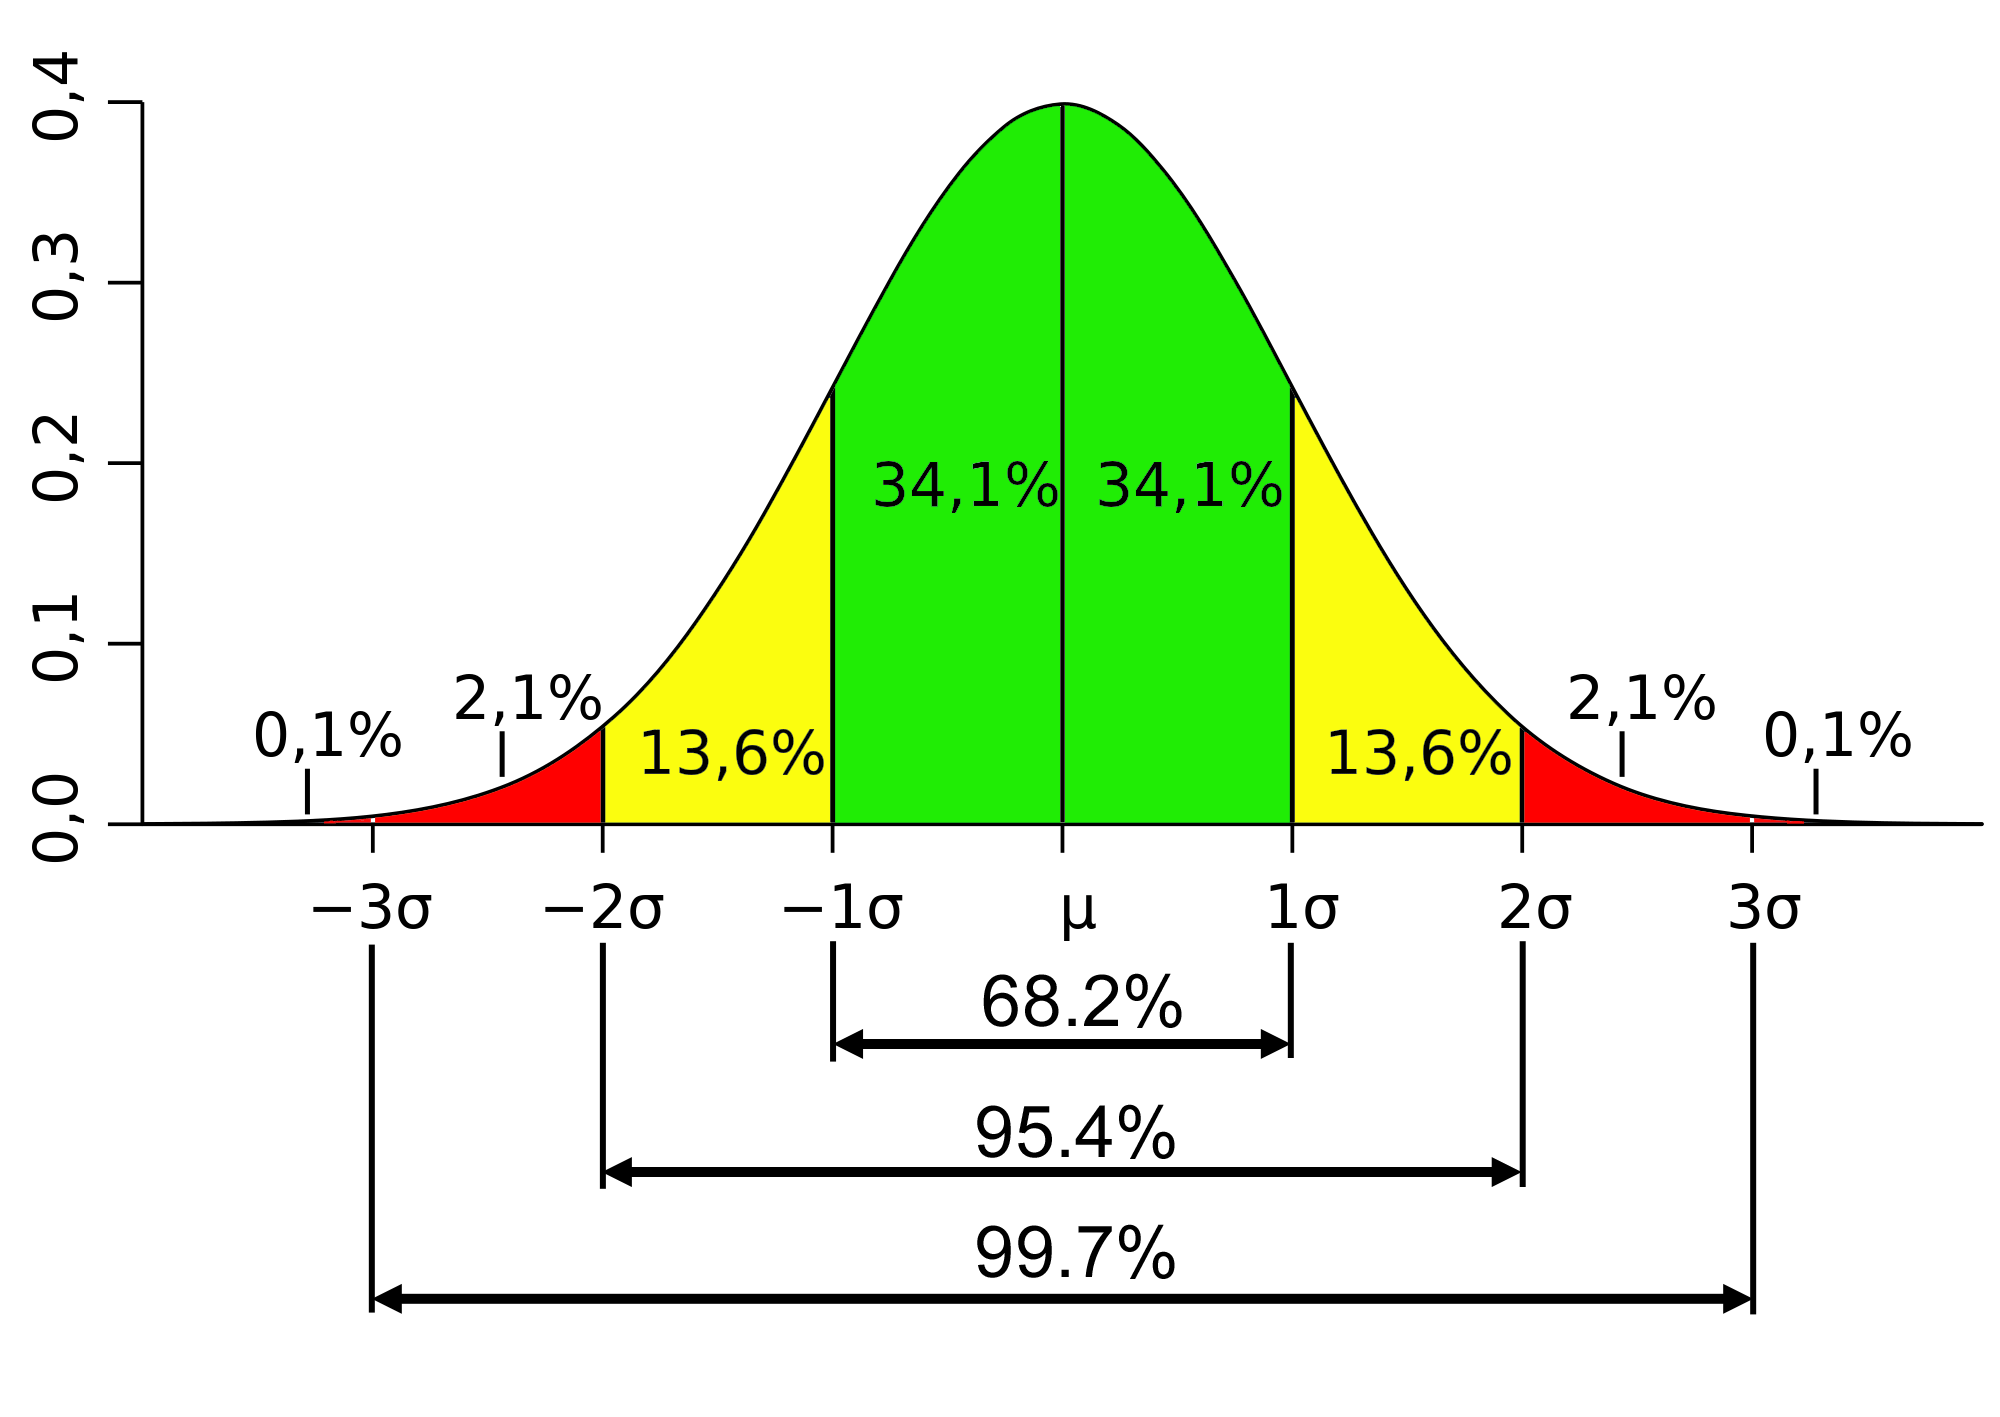
\includegraphics[width=0.6\textwidth]{/0225.png} \\	
			
		这些曲线下各段面积, 就是区间的概率. \\
		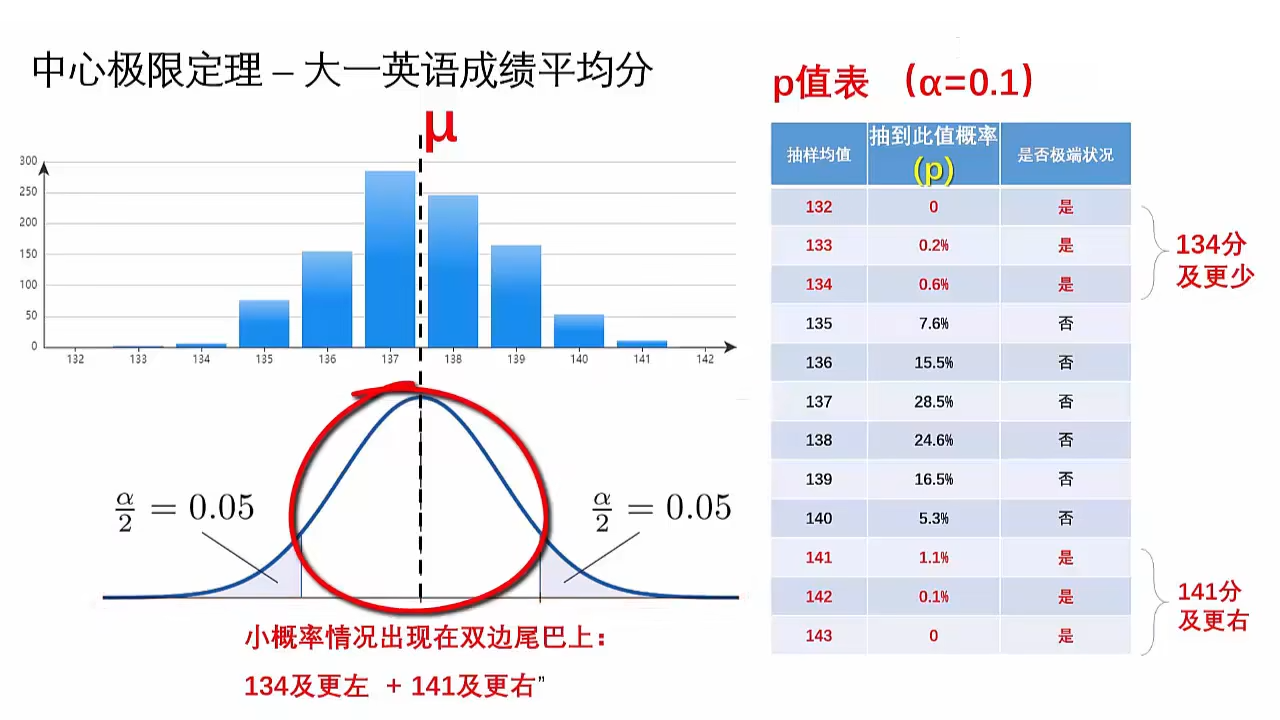
\includegraphics[width=1\textwidth]{/0226.png}		
	\end{myEnvSample}

	
	
	
	
	
	\section{(1) 原假设$H_0$ (null hypothesis), (2) 对立(或备选)的假设 $H_1$ (alternative hypothesis)}
	
	\begin{myEnvSample}
		我们有大一5000名学生的成绩表, 并知道 平均值$\mu$=137.41分. \\
		但我们不知道大四5000名学生的成绩表. 只能从中抽样, \textbf{并且只能抽样一次}. 那么, 我们如何知道大四的平均成绩呢?
		
		我们的思路是: 看看从大四中抽样的样本, 其``均值"是否能融入大一数据的正态分布世界中. 如果``大概率"地能融合进去, 则我们就可以``大概率"地判定, 大四数据的``正态分布世界", 和大一的``正态分布世界", 是一样的. 则两者的均值也相同. \\
		
		下面来具体操作: \\
		首先, 我们假设, 大四的平均分, 和大一的平均分是一样的. \textbf{我们把这个假设, 称为``原假设", 记为 $H_0$,  H 就是 hypothesis 的首字母.} \\
		
		也就是说, 大四成绩的``正态分布曲线", 我们先假设和大一的``正态分布曲线"形状是一样(属于同一个正态分布世界中). 如果这个原假设$H_0$ 是成立的话, 则, 虽然我们只能对大四抽样一次, 但该样本的均值, 依然会有95.4\%的可能性, 会落在大一的平均值$\mu$左右两侧``$2 \sigma$范围"的区间中. \\
		
		下面, 我们就来看看, 从大四样本中得到的均值实际数字, 是支持你上面的$H_0$呢? 还是不支持(即推翻)该假设呢? \\
		
		现在, 我们对大四的成绩, 抽样一次, 得到平均值是 141.3分. \\
		我们来看, 这个x=141.3, 在大一的正态分布曲线上, 处于什么位置和概率上? \\
		
		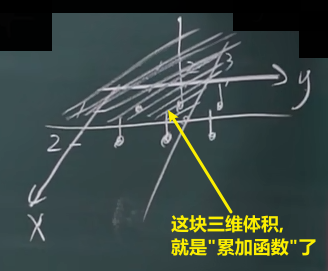
\includegraphics[width=0.9\textwidth]{/0227.png} \\
		
		\textbf{你发现, $P\{X\ge 141.3\}=1.2\%$, 说明这个数字出现在``大一的正态分布世界"中的概率, 极小. 是个小概率事件. 所以, 大四的这个数字, 就更可能属于别的正态分布世界中, 而不属于``大一的正态分布世界"中.} 要从``大一的正态分布世界"中踢出去. \\
		
		所以, 我们推翻了\textbf{原假设$H_0$ (null hypothesis)} (两个年级有相同的正态世界). 转而支持其\textbf{对立(或备选)的假设 $H_1$ (alternative hypothesis)} (两个年级的正态世界, 完全不同)
	\end{myEnvSample}
	
	
	
	
	
	
	\section{t检验}
	
	\begin{myEnvSample}
		
	\end{myEnvSample}
	
	
	
	
	
\end{document}